\documentclass[nooutcomes]{ximera}
%% handout
%% space
%% newpage
%% numbers
%% nooutcomes

%I added the commands here so that I would't have to keep looking them up
%\newcommand{\RR}{\mathbb R}
%\renewcommand{\d}{\,d}
%\newcommand{\dd}[2][]{\frac{d #1}{d #2}}
%\renewcommand{\l}{\ell}
%\newcommand{\ddx}{\frac{d}{dx}}
%\everymath{\displaystyle}
%\newcommand{\dfn}{\textbf}
%\newcommand{\eval}[1]{\bigg[ #1 \bigg]}

%\begin{image}
%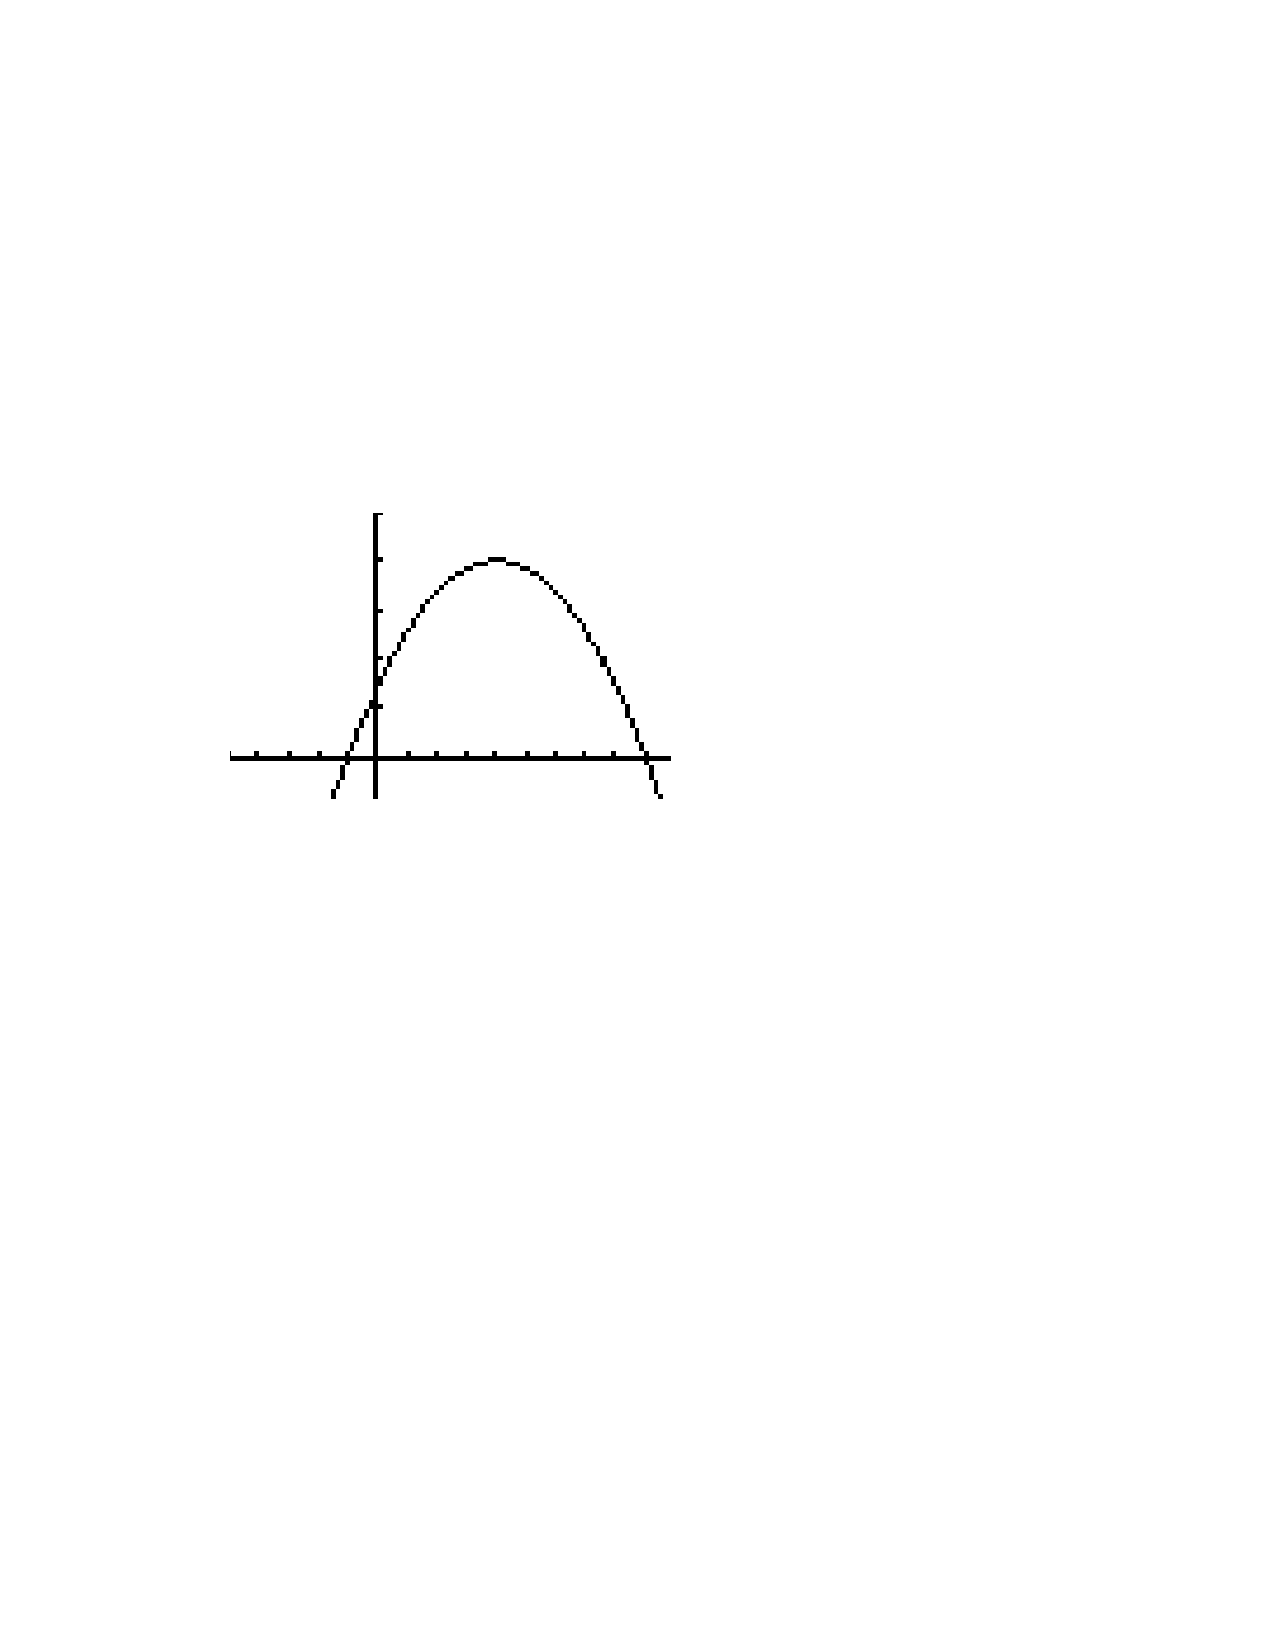
\includegraphics[trim= 170 420 250 180]{Figure1.pdf}
%\end{image}


\newcommand{\RR}{\mathbb R}
\renewcommand{\d}{\,d}
\newcommand{\dd}[2][]{\frac{d #1}{d #2}}
\renewcommand{\l}{\ell}
\newcommand{\ddx}{\frac{d}{dx}}
\newcommand{\dfn}{\textbf}
\newcommand{\eval}[1]{\bigg[ #1 \bigg]}

\usepackage{multicol}

\renewenvironment{freeResponse}{
\ifhandout\setbox0\vbox\bgroup\else
\begin{trivlist}\item[\hskip \labelsep\bfseries Solution:\hspace{2ex}]
\fi}
{\ifhandout\egroup\else
\end{trivlist}
\fi} %% we can turn off input when making a master document

\title{Recitation \#26 - 5.4 Working With Integrals (Solutions)}  

\begin{document}
\begin{abstract}		\end{abstract}
\maketitle

\section*{Warm up:} 
	\begin{enumerate}
		
	%part 1
	\item[1.]  If $f$ is an odd function, why is it true that $\int_{-a}^a f(x) \d x = 0$?  
	Support your reasoning with a picture.
		\begin{freeResponse}
		If $f$ is odd, then the regions between the graph of $f$ and the $x$-axis from $[-a,0]$ and $[0,a]$ are reflections of each other through the origin.  Thus, these two regions will have the same area but with opposite signs since they are on opposite sides of the $x$-axis.  They will therefore cancel each other out.
		
			\begin{image}
			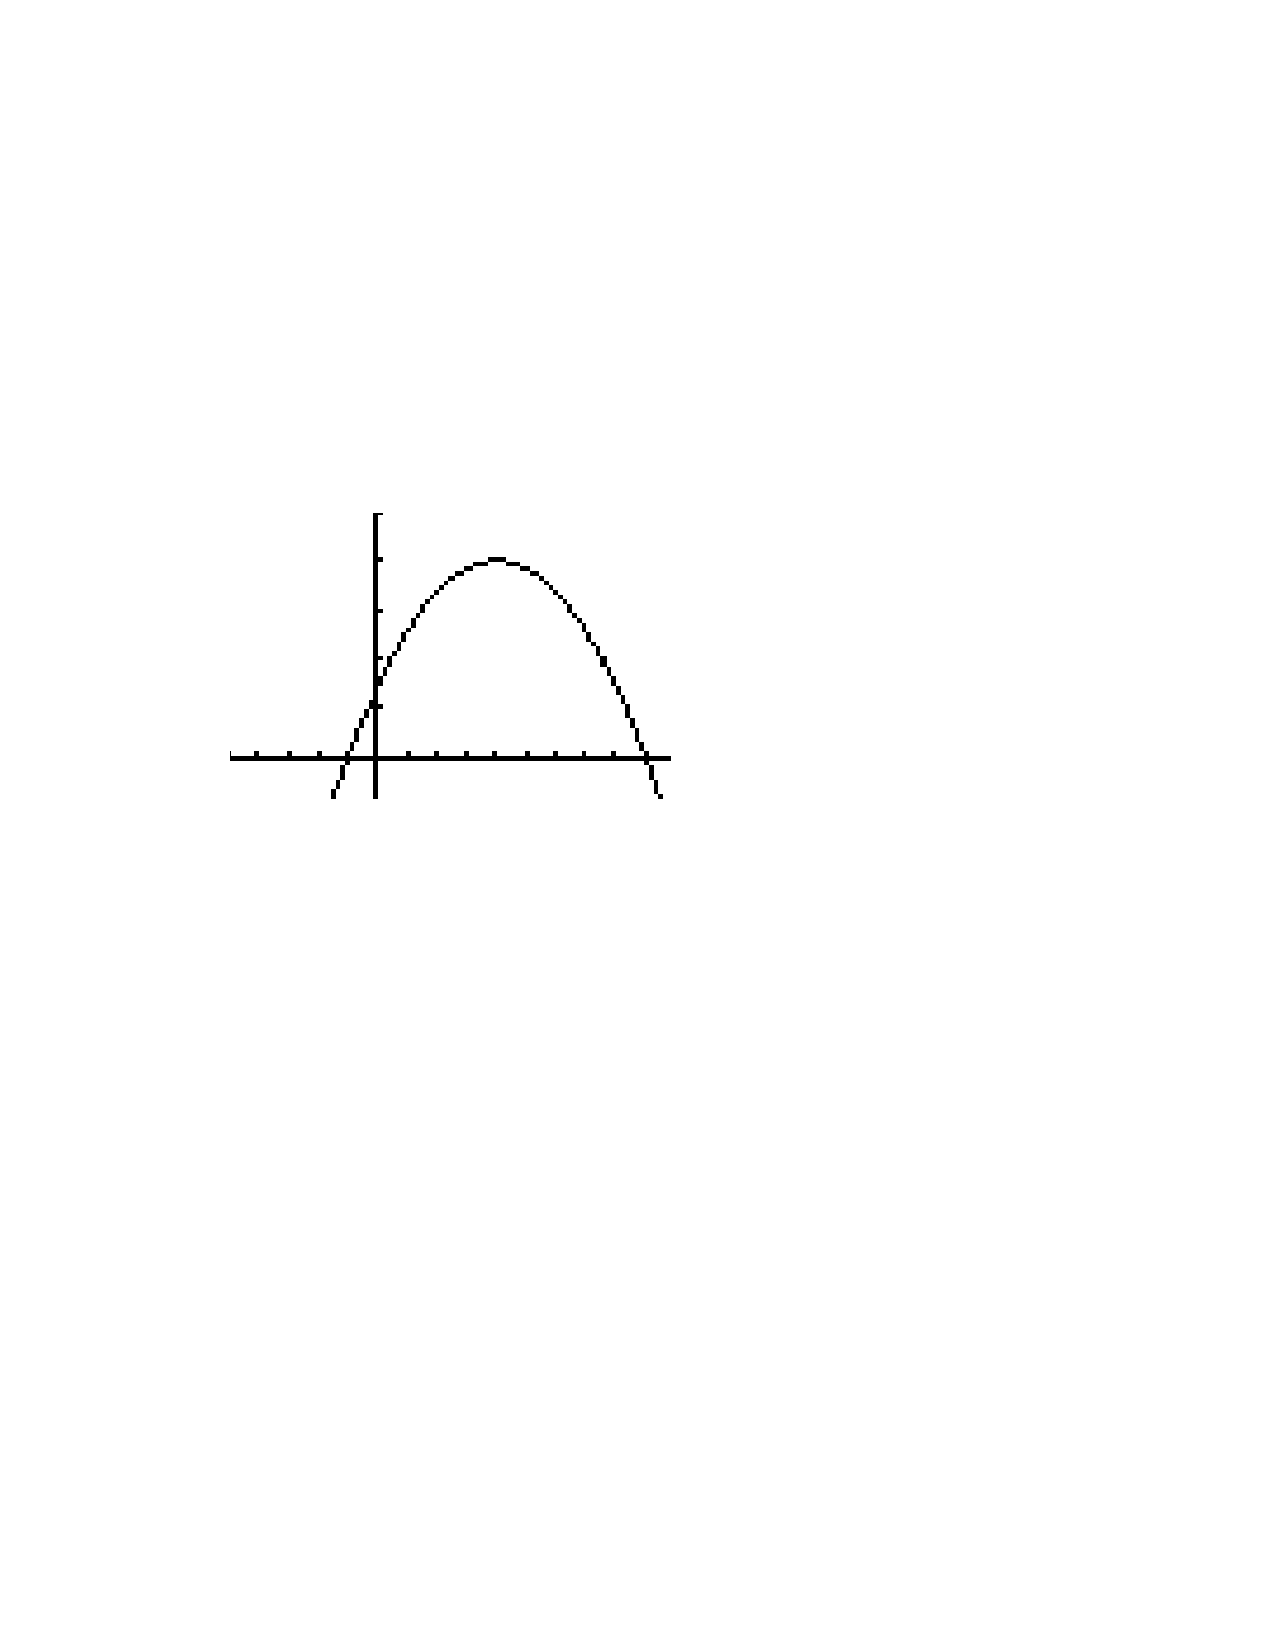
\includegraphics[trim= 170 440 250 200]{Figure1.pdf}
			\end{image}

		\end{freeResponse}	
		
		
		
	%part 1
	\item[2.]  If $f$ is an even function, why is it true that $\int_{-a}^a f(x) \d x = 2 \int_0^a f(x) \d x$?  
	Support your reasoning with a picture.
		\begin{freeResponse}
		If $f$ is even, then the regions between the graph of $f$ and the $x$-axis from $[-a,0]$ and $[0,a]$ are reflections of each other through the $y$-axis.  
		Thus, these two regions will have the same area with the same sign since they are on the same sides of the $x$-axis.
		So you can only find one of these areas and then double it.
		
			\begin{image}
			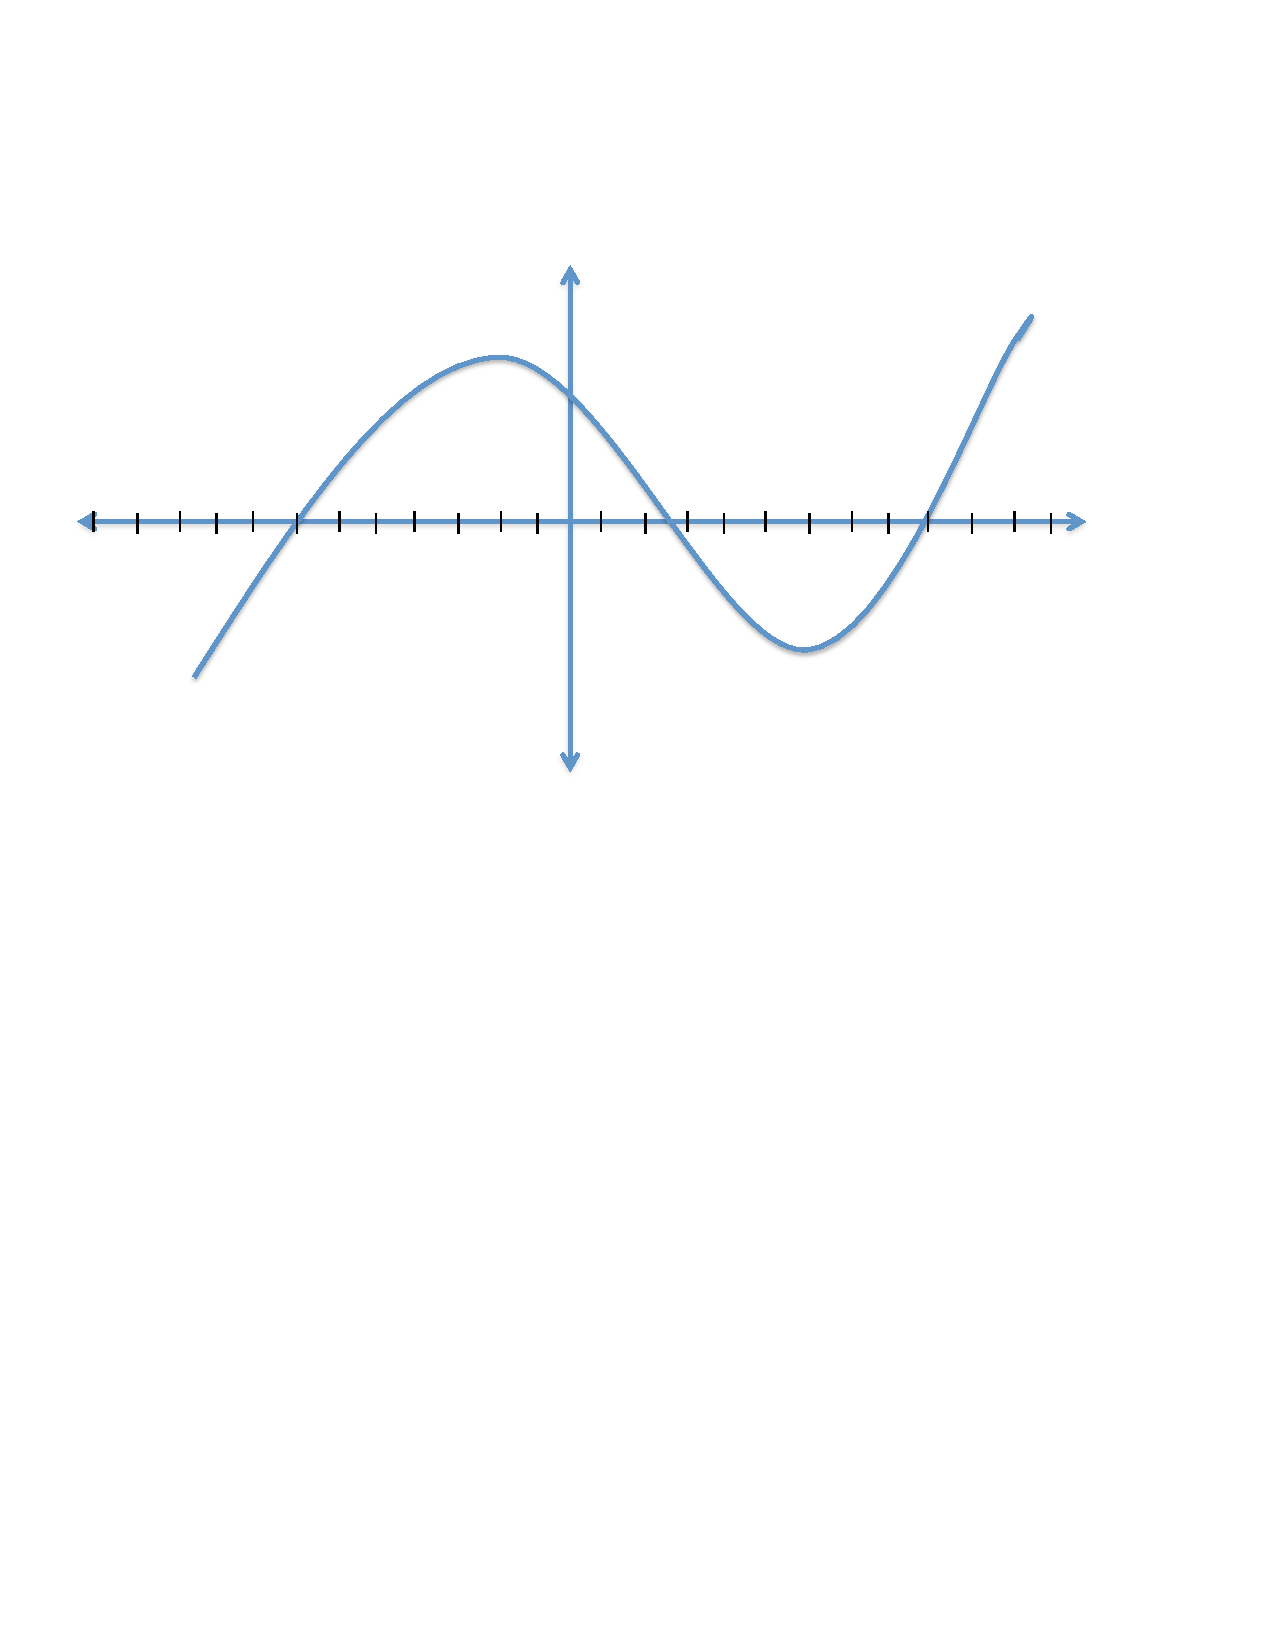
\includegraphics[trim= 170 430 250 200]{Figure2.pdf}
			\end{image}
			
		\end{freeResponse}	
		
		
		
	\end{enumerate}
		
		
		

	
	
	
	
	

\section*{Group work:}



%problem 1
\begin{problem}
\dfn{- Even and Odd Functions}
	\begin{enumerate}
	
	%part a
	\item  Find the following definite integral:
	\begin{equation*}
	\int_{-4}^4 \frac{x^2 \sin^3(x)}{\sqrt{x^4 + 1}} \d x
	\end{equation*}
		\begin{freeResponse}
		Let $f(x) = \frac{x^2 \sin^3(x)}{\sqrt{x^4 + 1}}$.  
		Then notice that
			\begin{align*}
			f(-x) &= \frac{(-x)^2 \sin^3(-x)}{\sqrt{(-x)^4 + 1}}  \\
			&= \frac{x^2 (- \sin(x))^3}{\sqrt{x^4 + 1}}  \quad \text{(since } \sin(x) \text{ is an odd function)}  \\
			&= \frac{- x^2 \sin^3(x)}{\sqrt{x^4 + 1}}  \\
			&= -f(x).
			\end{align*}
		Thus, $f$ is an odd function and therefore
			\begin{equation*}
			\int_{-4}^4 \frac{x^2 \sin^3(x)}{\sqrt{x^4 + 1}} \d x = 0.
			\end{equation*}
		\end{freeResponse}
		
		
		
	%part b
	\item  Suppose that $f$ is an even function.  Given that $\int_0^6 f(x) \d x = 13$, find $\int_{-6}^6 (5f(x) + 14) \d x$.
		\begin{freeResponse}
		First notice that
			\begin{equation}\label{linear integral}
			\int_{-6}^6 (5f(x) + 14) \d x = 5 \int_{-6}^6 f(x) \d x + \int_{-6}^6 14 \d x.
			\end{equation}
			
		Since $f$ is even, we know that
			\begin{equation}\label{int of f}
			\int_{-6}^6 f(x) \d x = 2 \int_0^6 f(x) \d x = 2 (13) = 26.
			\end{equation}
			
		We also know that
			\begin{equation}\label{int of 14}
			\int_{-6}^6 (5f(x) + 14) \d x = \eval{14x}_{-6}^6 = 14(6 - (-6)) = 14(12) = 168.
			\end{equation}
			
		Then substituting equations \eqref{int of f} and \eqref{int of 14} into equation \eqref{linear integral} gives:
			\begin{equation*}
			\int_{-6}^6 (5f(x) + 14) \d x = 5(26) + 168 = 130 + 168 = 298.
			\end{equation*}
		\end{freeResponse}
		
		
		
	\end{enumerate}
		
		
\end{problem}
















%problem 2
\begin{problem}
\dfn{- Average Value of a Function}
	\begin{enumerate}
	
	%part a
	\item  A cup of coffee has temperature $20 + 75e^{-.02t}$ degrees (Celsius) $t$ minutes after being poured into a cup.  
	What is the average temperature of the coffee during the first half hour?
		\begin{freeResponse}
		Let $T(t) := 20 + 75e^{-.02t}$.  We want the average value of $T$ on $[0,30]$.
			\begin{align*}
			T_{\text{avg}} &= \frac{1}{30-0} \int_0^{30} \left( 20 + 75e^{-.02t} \right) \d t  \\
			&= \frac{1}{30} \eval{20t - \frac{75}{.02} e^{-.02t}}_0^{30}  \\
			&= \frac{1}{30} \eval{20t - 3750 e^{-.02t}}_0^{30}  \\
			&= \frac{1}{30} \left[ \left( 20(30) - 3750e^{-0.6} \right) - (0 - 3750) \right]  \\
			&= \frac{1}{30} \left( 4350 - 3750e^{-0.6} \right)  \\
			&= 145 - 125e^{-0.6} 
			\end{align*}
		So the average temperature of the coffee during the half hour is $145 - 125e^{-0.6}$ degrees Celsius.
		\end{freeResponse}
		
		
		
	%part b
	\item  Let $A$ denote the average value of $\sin(x)$ over the interval $[0,1000]$, 
	and let $B$ denote the average value of $\sin^2(x)$ over that same interval.  
	Use basic reasoning to determine which is greater:  $A^2$ or $B$?  
		\begin{freeResponse}
		$A \approx 0$ since $\sin(x)$ is evenly above and below the $x$-axis over $[0,1000]$.  
		So then $A^2 < A$.  
		$\sin^2(x)$ is close to being evenly distributed between $0$ and $1$, and so its average value ($B$) should be close to $1/2$.  
		Therefore, $A^2 < B$
		\end{freeResponse}
		
		
		
	\end{enumerate}
		
		
		

\end{problem}
	
	
	
	
	
	
	
	
			
			

%problem 3
\begin{problem}
\dfn{- Mean Value Theorem for Integrals}

Find all points at which the given function equals its average value on the given interval.
	\begin{enumerate}
	
	%part a
	\item  $f(x) = e^x	\qquad	[0,4]$
		\begin{freeResponse}
		First, we need to find $f_{\text{avg}}$:
			\begin{align*}
			f_{\text{avg}} &= \frac{1}{4-0} \int_0^4 e^x \d x  \\
			&= \frac{1}{4} \eval{e^x}_0^4  \\
			&= \frac{1}{4} \left( e^4 - 1 \right)  
			\end{align*}
		So we are looking for all values $c \in [0,4]$ such that:
			\begin{align*}
			f(c) &= \frac{1}{4} (e^4 - 1)  \\
			\Longrightarrow \quad e^c &= \frac{1}{4} (e^4 - 1)  \\
			\Longrightarrow \quad c &= \ln \left( \frac{1}{4} (e^4 - 1) \right)
			\end{align*}
		Therefore, our answer is $\ln \left( \frac{1}{4} (e^4 - 1) \right)$.
		\end{freeResponse}
		
		
		
	%part b
	\item  $g(x) = \frac{\pi}{4} \sin(x)	\qquad	[0,\pi]$
		\begin{freeResponse}
		First, we need to find $g_{\text{avg}}$:
			\begin{align*}
			g_{\text{avg}} &= \frac{1}{\pi-0} \int_0^{\pi} \frac{\pi}{4} \sin(x) \d x  \\
			&= \frac{1}{4} \eval{-\cos(x)}_0^{\pi}  \\
			&= \frac{1}{4} \left( - (-1-1) \right)  \\
			&= \frac{1}{2}
			\end{align*}
		So we are looking for all values $c \in [0,\pi]$ such that:
			\begin{align*}
			&g(c) = \frac{1}{2}  \\
			&\Longrightarrow \quad \frac{\pi}{4} \sin(c) = \frac{1}{2}  \\
			&\Longrightarrow \quad \sin(c) = \frac{2}{\pi}  \\
			&\Longrightarrow \quad c = \arcsin \left( \frac{2}{\pi} \right), \pi - \arcsin \left( \frac{\pi}{2} \right)
			&\end{align*}
		Therefore, our two answers are $\arcsin \left( \frac{2}{\pi} \right), \pi - \arcsin \left( \frac{\pi}{2} \right)$.
		\end{freeResponse}
		
		
		
	\end{enumerate}
			
			
		
\end{problem}


















	
	
	
	
	
	
	
	
	

	










								
				
				
	














\end{document} 


















